\documentclass{article}
\usepackage[english]{babel}
\usepackage[utf8]{inputenc}
\usepackage{fancyhdr}
\usepackage{amsmath}
\usepackage{pdfpages}

\pagestyle{fancy}
\fancyhf{}
\rhead{CS760}
\lhead{Cheng-Wei Lu}
\rfoot{Page \thepage}

\begin{document}

\section*{CS 760 Homework 1 by Cheng-Wei Lu}

\subsection*{Problem 1.1}
	Suppose there are two vectors $u,v \in R^D$, and $a,b \in R$.
	\begin{equation*}
		u= \begin{pmatrix} x_1 \\ . \\ . \\ . \\ x_D \end{pmatrix},  v= \begin{pmatrix} y_1 \\ . \\ . \\ . \\ y_D \end{pmatrix}.     x_n, y_n \in R, \forall n = 1 ... D. 
	\end{equation*}
	\begin{equation*}
		au + bv =  \begin{pmatrix} ax_1 + by_1\\ . \\ . \\ . \\ ax_D+by_D \end{pmatrix} \in R^D \subseteq R^D 
	\end{equation*}
	\textbf{Q.E.D}

\subsection*{Problem 1.2}
    \subsubsection*{(a)}	
    	Suppose $u \in R^D$,
    	 \begin{equation*}
    		u= \begin{pmatrix} x_1 \\ . \\ . \\ . \\ x_D \end{pmatrix}, x_n \in R, \forall n = 1 ... D. 
    	\end{equation*}
    	Suppose $x_1 <  0$, element-wise square root of $u$
    	
    	 \begin{equation*}
    		= \begin{pmatrix} \sqrt{x_1} \\ . \\ . \\ . \\ \sqrt{x_D} \end{pmatrix} \notin R^D, \text{since  $\sqrt{x_1}$ is not a real number} 
    	\end{equation*}
    	\textbf{Q.E.D}
    \subsubsection*{(b)}
    	$0^D$ is closed under element-wise square root, and is a subspace for $R^D$. Suppose $u \in 0^D$,
    	 \begin{equation*}
    		u= \begin{pmatrix} x_1 \\ . \\ . \\ . \\ x_D \end{pmatrix} = \begin{pmatrix} 0 \\ . \\ . \\ . \\ 0 \end{pmatrix},
    	\end{equation*}
	element-wise square root of $u$
	 \begin{equation*}
    		= \begin{pmatrix} \sqrt{0} \\ . \\ . \\ . \\ \sqrt{0} \end{pmatrix}  = \begin{pmatrix} 0 \\ . \\ . \\ . \\ 0 \end{pmatrix} \in 0^D,
    	\end{equation*}

and if there is another $v \in 0^D$,
	\begin{equation*}
		au + bv = a \begin{pmatrix} 0 \\ . \\ . \\ . \\ 0 \end{pmatrix} + b \begin{pmatrix} 0 \\ . \\ . \\ . \\ 0 \end{pmatrix}  =  \begin{pmatrix} 0 \\ . \\ . \\ . \\ 0 \end{pmatrix} \in 0^D.
	\end{equation*}
	\textbf{Q.E.D}

\subsection*{Problem 1.3}
	Suppose there are two vectors $w,v \in U$,
	
	 \begin{equation*}
    		w= \sum_{i=1}^{R} a_iu_i, \text{and  } v= \sum_{i=1}^{R} b_iu_i, \text{where } a_i,b_i\in R,\forall i, i = 1...R.
	\end{equation*}
	
	 \begin{equation*}
    		xw + yv= \sum_{i=1}^{R}(xa_i+yb_i)u_i \in U, \text{where } x,y_i\in R.
	\end{equation*}
\textbf{Q.E.D}

\subsection*{Problem 1.4}
\subsubsection*{(a)}
	\begin{equation*}
		P(diabetes | inactive) = \frac{P(inactive|diabetes)\times P(diabetes)}{P(inactive)} =  \frac{9.3\% \times 95\%}{P(inactive)}
	\end{equation*}

\subsubsection*{(b)}
	I still need to know the portion of the population who has the 3 genes inactive.

\subsubsection*{(c)}
	If the portion of the population who has the 3 genes inactive is low, then I should be concerned.
	
\subsection*{Problem 1.5}
	I think the distribution can be the right half of normal distribution times 2, where $\mu = t_0$ and $\sigma = \theta$.
	\begin{equation*}
		X\sim N(\mu = t_0,\sigma = \theta)
	\end{equation*}
	
	To be more specific,

        \[ P(x|\theta)=\begin{cases} 
              \frac{2}{ \theta \sqrt{2\pi}}e^{\frac{-1}{2}}(\frac{x-t_0}{\theta}) &, x\geq t_0, \\
              0 &, x<t_0. 
           \end{cases}
        \]
	
	Note that $\int_{t_0}^{\infty} \frac{2}{ \theta \sqrt{2\pi}}e^{\frac{-1}{2}}(\frac{x-t_0}{\theta}) \text{  }dx = 1$.
	I choose normal distribution because, as described in the problem, the probability of delay time is strictly decreasing as delay time grows, which is also the case of the right half of a normal distribution.
	
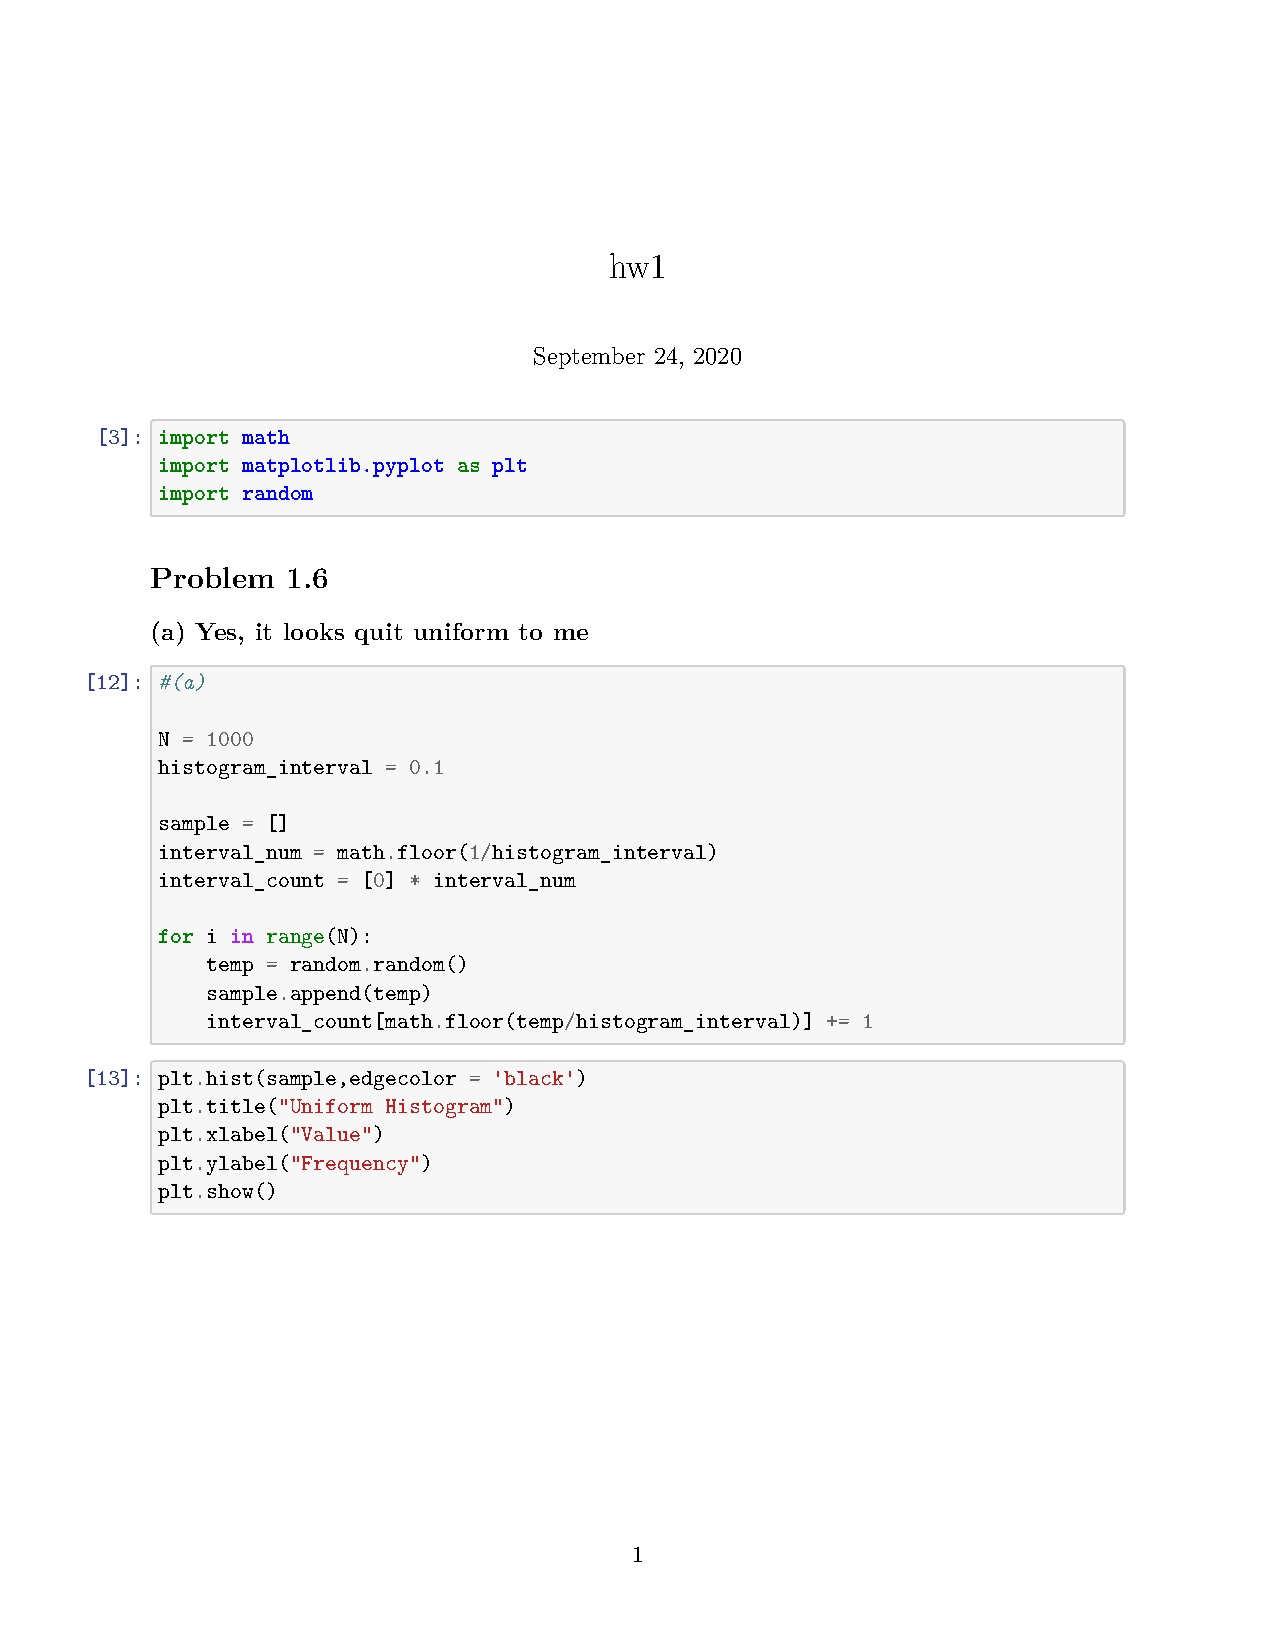
\includepdf[page={1,2,3,4,5,6}]{hw1-2.pdf}
	
\subsection*{Problem 1.7}
\subsubsection*{(a)}
	\begin{equation*}
		l(\theta) = \sum_{i=1}^{N} y_ilog((\frac{1}{1+e^{-\theta^T x_i}})) + (1-y_i)log(1-(\frac{1}{1+e^{-\theta^Tx_i}})) 
	\end{equation*}
	

		\begin{equation*}
		\begin{aligned}
    		\frac{\partial l(\theta)}{\partial \theta^T} = \sum_{i=1}^{N} y_i(1+e^{-\theta^Tx_i})\times \frac{e^{-\theta^Tx_i}\times x_i}{(1+e^{-\theta^Tx_i})^2}  + (1-y_i) \times \frac{1+e^{-\theta^Tx_i}}{e^{-\theta^Tx_i}} &&\\ 
		 \times \frac{e^{-\theta^Tx_i}\times (-x_i)(1+e^{-\theta^Tx_i})-e^{-\theta^Tx_i} \times (-x_i)\times e^{-\theta^Tx_i}}{(1+e^{-\theta^Tx_i})^2 } \\
		 = \sum_{i=1}^{N}y_i \times \frac{e^{-\theta^Tx_i}}{1+e^{-\theta^Tx_i}}x_i + (y_i-1)\frac{1}{1+e^{-\theta^Tx_i}}x_i \\
		 = \sum_{i=1}^{N}y_i\times x_i - \frac{1}{e^{-\theta^Tx_i }}x_i\\
		\underline{ \underline{=\sum_{i=1}^{N}x_i(y_i-\frac{1}{e^{-\theta^Tx_i}})}}
		\end{aligned}
		\end{equation*}
\subsubsection*{(b)}
	\begin{equation*}
		\begin{aligned}
			\frac{\partial l(\theta)}{\partial \theta \partial \theta^T}  = \sum_{i=1}^{N} -x_i(\frac{-e^{-\theta^Tx_i}\times (-x_i^T)\times 1}{(1+e^{-\theta^Tx_i})^2}) \underline{ \underline{ = \sum_{i=1}^{N}\frac{-e^{-\theta^Tx_i}}{(1+e^{-\theta^Tx_i})^2}x_ix_i^T}}
		\end{aligned}
	\end{equation*}

\subsubsection*{(c)}
	$l(\theta)$ is a scalar, gradient is a vector, and Hessian is a matrix.
	 

\end{document}


